\documentclass[aspectratio=169, table, 12pt]{beamer}

\usepackage{colortbl}
\usepackage{xcolor}
\usepackage{listings}
\usepackage{tabularx}
\usepackage{tikz}
\usetikzlibrary{arrows.meta, positioning, calc, fit, shapes.geometric}

\makeatletter
\def\input@path{{../theme/}}
\makeatother
\graphicspath{{../theme/}{../../figures/}}
\usetheme{Pradita}

\definecolor{praditagreen}{RGB}{37, 113, 71}

% Tema membuat garis tabel berwarna putih. Dikembalikan agar tabel terbaca.
\arrayrulecolor{black}
\setlength{\arrayrulewidth}{0.5pt}

% Kolom X rata kiri, dipakai pada tabel dengan kolom X yang sempit, agar
% spasi antarkata tidak meregang.
\newcolumntype{Y}{>{\raggedright\arraybackslash}X}

\lstdefinelanguage{bash}{
  keywords={},
  basicstyle=\ttfamily\scriptsize,
  ndkeywords={cd, coverage, curl, diff, docker, echo, npm, npx, python,
              python3, pytest, source},
  ndkeywordstyle=\color{purple}\bfseries,
  sensitive=true,
  commentstyle=\color{gray},
  numbers=none,
  breaklines=true,
  frame=lines,
  backgroundcolor=\color{lightgray!10},
  tabsize=2,
  comment=[l]{\#},
  showstringspaces=false
}

\lstdefinelanguage{TypeScript}{
  keywords={const, let, function, return, async, await, try, catch, throw,
            new, if, interface, void, export, import, from, type},
  ndkeywords={Promise, number, string, boolean, test, expect, Page, await},
  basicstyle=\ttfamily\scriptsize,
  keywordstyle=\color{blue}\bfseries,
  ndkeywordstyle=\color{purple}\bfseries,
  sensitive=true,
  commentstyle=\color{gray}\itshape,
  stringstyle=\color{red},
  numbers=none,
  breaklines=true,
  frame=lines,
  backgroundcolor=\color{lightgray!10},
  tabsize=2,
  comment=[l]{//},
  morestring=[b]",
  showstringspaces=false
}

% Gaya Python disamakan dengan naskah bab, tanpa nomor baris.
\lstdefinestyle{PythonStyle}{
  language=Python,
  basicstyle=\ttfamily\scriptsize,
  morekeywords={with, as, yield, async, await, match, case},
  keywordstyle=\color{blue}\bfseries,
  emph={pytest, psycopg, Mock, given, strategies},
  emphstyle=\color{purple}\bfseries,
  commentstyle=\color{gray}\itshape,
  stringstyle=\color{red},
  numbers=none,
  breaklines=true,
  frame=lines,
  backgroundcolor=\color{lightgray!10},
  tabsize=2,
  showstringspaces=false
}

% File mutu dan kontrak ditampilkan apa adanya, sehingga butuh gaya JSON.
\lstdefinelanguage{json}{
  basicstyle=\ttfamily\scriptsize,
  stringstyle=\color{red},
  commentstyle=\color{gray},
  numbers=none,
  breaklines=true,
  frame=lines,
  backgroundcolor=\color{lightgray!10},
  tabsize=2,
  showstringspaces=false,
  morestring=[b]"
}

\title{\Huge Keamanan\\ \vspace{10pt} Aplikasi Web}
\subtitle{IF140303 - Pengembangan Aplikasi Web}
\author{\textbf{Alfa Yohannis}}

\begin{document}

\frame{\titlepage}

\begin{frame}[fragile]
  \frametitle{Isi Pertemuan}
  \vspace{14pt}
  \begin{columns}[t]
    \column{0.5\textwidth}
    {\small\tableofcontents[sections={1-7}]}

    \column{0.5\textwidth}
    {\small\tableofcontents[sections={8-14}]}
  \end{columns}
\end{frame}

\begin{frame}{\hfill}
  \centering
  \Huge{\textbf{Apa yang terjadi bila aplikasi ini\\dipakai di luar niat pembuatnya?}}
\end{frame}

\section{Tujuan dan Kerangka Bahasan}

\begin{frame}{\hfill}
  \centering
  \Huge{\textbf{Tujuan dan Kerangka Bahasan}}
\end{frame}

\begin{frame}{{\Large Tujuan Pembelajaran}}
  \vspace{10pt}
  \begin{itemize}
    \item Menyusun model ancaman satu aplikasi web, yaitu menyebut batas
          kepercayaannya, data yang bernilai, dan jalan masuk yang tersedia.
    \item Memasang pertahanan bawaan di sisi server, lalu membuktikan
          terpasangnya dari \textit{response} yang dikirim aplikasi.
    \item Mengukur keamanan sebagai angka, yaitu jumlah syarat yang terpenuhi
          dan jumlah kerentanan dependensi, lalu menegakkannya sebagai
          \textit{gate}.
  \end{itemize}
\end{frame}

\begin{frame}{{\Large Jawaban Disusun Terbalik}}
  \vspace{12pt}
  \begin{itemize}
    \item Jumlah cara memakai aplikasi di luar niat pembuatnya jauh lebih
          banyak daripada jumlah cara memakainya dengan benar.
    \item Karena itu pertahanannya dipasang sebagai bawaan, lalu
          keberadaannya diperiksa ulang pada tiap perubahan.
  \end{itemize}
  \vspace{10pt}
  {\small Keamanan pindah dari ingatan orang ke file yang dapat dibaca mesin,
  persis seperti \textit{budget} performa Bab 5 dan batas mutu Bab 6. Seluruh
  pemeriksaan di sini bersifat mengamati, dan sasarannya aplikasi sendiri di
  komputer sendiri.}
\end{frame}

\section{Threat Modelling}

\begin{frame}{\hfill}
  \centering
  \Huge{\textbf{Threat Modelling}}
\end{frame}

\begin{frame}{{\Large Batas Kepercayaan}}
  \vspace{8pt}
  \centering
  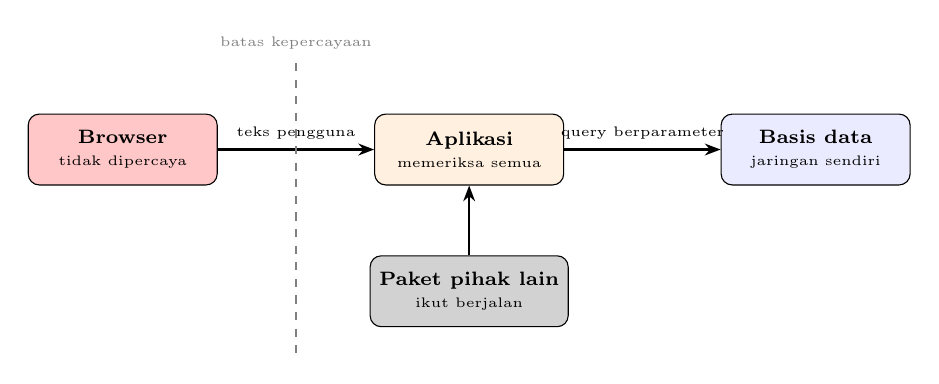
\begin{tikzpicture}[
    font=\scriptsize,
    kotak/.style={draw, rounded corners, minimum height=0.9cm,
                  minimum width=2.4cm, align=center, font=\scriptsize\bfseries},
    panah/.style={-{Stealth[length=2mm]}, thick}
  ]
    \node[kotak, fill=red!22] (browser) at (0,0) {Browser\\{\tiny\mdseries tidak dipercaya}};
    \node[kotak, fill=orange!12] (server) at (4.4,0) {Aplikasi\\{\tiny\mdseries memeriksa semua}};
    \node[kotak, fill=blue!8] (basis) at (8.8,0) {Basis data\\{\tiny\mdseries jaringan sendiri}};
    \node[kotak, fill=gray!35] (paket) at (4.4,-1.8) {Paket pihak lain\\{\tiny\mdseries ikut berjalan}};

    \draw[panah] (browser) -- node[font=\tiny, above] {teks pengguna} (server);
    \draw[panah] (server) -- node[font=\tiny, above] {query berparameter} (basis);
    \draw[panah] (paket) -- (server);
    \draw[dashed, thick, gray] (2.2,1.1) -- (2.2,-2.6);
    \node[font=\tiny, gray, anchor=south] at (2.2,1.15) {batas kepercayaan};
  \end{tikzpicture}

  \vspace{8pt}
  {\small Yang ditulis lebih dahulu bukan daftar serangan, melainkan daftar
  pintu: di mana data berpindah tangan, dan siapa yang dipercaya di tiap
  sisinya.}
\end{frame}

\begin{frame}{{\Large Tiga Kewajiban yang Keluar dari Gambar Itu}}
  \vspace{14pt}
  \begin{enumerate}
    \item Teks dari browser tidak pernah disambung langsung ke dalam perintah
          apa pun.
    \item \textit{Response} membawa aturan main untuk browser, yaitu header
          keamanan dan atribut cookie.
    \item Paket pihak lain ikut dihitung sebagai jalan masuk, sehingga
          daftarnya diperiksa berkala.
  \end{enumerate}
  \vspace{10pt}
  {\small Ketiganya yang dibuktikan satu per satu di sisa pertemuan ini.}
\end{frame}

\section{Header Keamanan}

\begin{frame}{\hfill}
  \centering
  \Huge{\textbf{Header Keamanan}}
\end{frame}

\begin{frame}{{\Large Server Bawaan lawan Aplikasi yang Dikeraskan}}
  \vspace{6pt}
  \centering
  {\footnotesize
  \begin{tabularx}{\textwidth}{Yll}
    \hline
    \textbf{Header} & \textbf{Server bawaan} & \textbf{Aplikasi Bab 7} \\
    \hline
    \texttt{Content-Security-Policy} & tidak ada & \texttt{default-src 'self'} \\
    \hline
    \texttt{X-Content-Type-Options} & tidak ada & \texttt{nosniff} \\
    \hline
    \texttt{Referrer-Policy} & tidak ada & \texttt{no-referrer} \\
    \hline
    \texttt{Permissions-Policy} & tidak ada & \texttt{geolocation=(), camera=()} \\
    \hline
  \end{tabularx}}

  \vspace{8pt}
  {\small Keduanya diukur dengan \texttt{curl} di komputer yang sama. Header
  keamanan tidak datang sendiri: server statis bawaan Python tidak mengirim
  satu pun.}
\end{frame}

\begin{frame}{{\Large Apa yang Dijaga Masing-Masing}}
  \vspace{12pt}
  \begin{itemize}
    \item \texttt{Content-Security-Policy} membatasi asal skrip dan gambar
          yang boleh dimuat halaman.
    \item \texttt{X-Content-Type-Options} menutup kebiasaan browser menebak
          jenis file dari isinya.
    \item \texttt{Referrer-Policy} menahan alamat halaman asal agar tidak
          ikut terkirim ke situs lain.
    \item \texttt{Permissions-Policy} mematikan kemampuan perangkat yang
          memang tidak dipakai: lokasi, kamera, mikrofon.
  \end{itemize}
\end{frame}

\begin{frame}[fragile]{{\Large Dipasang di Satu Tempat}}
  \vspace{2pt}
\begin{lstlisting}[style=PythonStyle]
  def kirim_response(self, status, isi_response, jenis_isi, header_tambahan):
    """Mengirim satu response lengkap beserta seluruh header keamanannya."""
    self.send_response(status)
    self.send_header("Content-Type", jenis_isi)
    self.send_header("Content-Length", str(len(isi_response)))
    for nama_header, nilai in self.server.kebijakan["header_wajib"].items():
      self.send_header(nama_header, nilai)
\end{lstlisting}
  \vspace{4pt}
  {\small Seluruh \textit{response} lewat fungsi ini, sehingga alamat baru
  tidak dapat lupa memasang headernya.}
\end{frame}

\section{Cookie yang Aman}

\begin{frame}{\hfill}
  \centering
  \Huge{\textbf{Cookie yang Aman}}
\end{frame}

\begin{frame}{{\Large Atribut Pembatas Cookie Sesi}}
  \vspace{6pt}
  \centering
  {\footnotesize
  \begin{tabularx}{\textwidth}{lY}
    \hline
    \textbf{Atribut} & \textbf{Yang dijaga} \\
    \hline
    \texttt{HttpOnly} & Cookie tidak dapat dibaca JavaScript mana pun di halaman \\
    \hline
    \texttt{SameSite=Lax} & Cookie tidak ikut terkirim pada permintaan yang dipicu situs lain \\
    \hline
    \texttt{Path=/} & Jangkauan cookie ditulis eksplisit, bukan ditebak browser \\
    \hline
    \texttt{Max-Age=3600} & Sesi berakhir sendiri sesudah satu jam \\
    \hline
  \end{tabularx}}

  \vspace{8pt}
  {\small \texttt{Secure} sengaja tidak dipasang, karena latihan berjalan
  lewat HTTP di \textit{localhost}. Pada aplikasi yang dilayani lewat HTTPS,
  atribut itu wajib ada.}
\end{frame}

\section{Aturan Lintas Origin}

\begin{frame}{\hfill}
  \centering
  \Huge{\textbf{Aturan Lintas Origin}}
\end{frame}

\begin{frame}{{\Large Dua Hal pada CORS Sering Tertukar}}
  \vspace{12pt}
  \begin{itemize}
    \item Izin \textit{Cross-Origin Resource Sharing} (CORS) menentukan
          siapa yang boleh \textbf{membaca} \textit{response}.
    \item Pemeriksaan hak akses menentukan siapa yang boleh \textbf{meminta}.
  \end{itemize}
  \vspace{10pt}
  {\small Yang dilindungi CORS adalah pembacanya, bukan servernya. Server
  tetap wajib memeriksa hak akses sendiri, karena permintaan dari luar
  browser tidak terikat aturan CORS sama sekali.}
\end{frame}

\begin{frame}{{\Large Izin Menurut Daftar, Bukan Kebetulan}}
  \vspace{6pt}
  \centering
  {\footnotesize
  \begin{tabularx}{\textwidth}{lY}
    \hline
    \textbf{Origin yang meminta} & \textbf{Header izin yang dikirim} \\
    \hline
    \texttt{https://toko.pradita.ac.id} & \texttt{Access-Control-Allow-Origin} berisi origin itu sendiri \\
    \hline
    \texttt{http://127.0.0.1:8030} & \texttt{Access-Control-Allow-Origin} berisi origin itu sendiri \\
    \hline
    \texttt{https://situs-lain.example} & tidak ada, hanya \texttt{Vary: Origin} \\
    \hline
  \end{tabularx}}

  \vspace{8pt}
  {\small Nilai bintang sengaja tidak dipakai: ia membuka \textit{response}
  bagi situs mana pun, dan menariknya kembali merusak halaman yang terlanjur
  bergantung padanya.}
\end{frame}

\section{Teks dari Pengguna}

\begin{frame}{\hfill}
  \centering
  \Huge{\textbf{Teks dari Pengguna}}
\end{frame}

\begin{frame}[fragile]{{\Large Dikirim sebagai Parameter}}
  \vspace{2pt}
\begin{lstlisting}[style=PythonStyle]
def cari_buku(judul_dicari):
  """Mencari buku menurut judulnya, dengan judul dikirim sebagai parameter.

  Teks dari pengguna tidak pernah disambung ke dalam SQL. Tanda kutip, tanda
  titik koma, dan kata kunci SQL di dalamnya diperlakukan sebagai data biasa,
  sehingga hasilnya hanya kosong, bukan perintah tambahan.
  """
  pola = f"%{judul_dicari}%"
  with psycopg.connect(DSN) as koneksi:
    baris = koneksi.execute(SQL_CARI_BUKU, (pola, BATAS_HASIL_CARI)).fetchall()
\end{lstlisting}
\end{frame}

\begin{frame}{{\Large Dua Pencarian, Satu Perlakuan}}
  \vspace{6pt}
  \centering
  {\footnotesize
  \begin{tabularx}{\textwidth}{Yrl}
    \hline
    \textbf{Kata kunci yang dikirim} & \textbf{Baris} & \textbf{Status} \\
    \hline
    \texttt{Pengantar Jilid 7} & 20 & 200, tanpa \textit{error} \\
    \hline
    \texttt{Pengantar'; SELECT 1 -{}-} & 0 & 200, tanpa \textit{error} \\
    \hline
  \end{tabularx}}

  \vspace{8pt}
  {\small Baris kedua nol bukan karena teksnya ditolak, melainkan karena
  tidak ada judul yang berisi rangkaian huruf itu. Bagi basis data, isinya
  tidak berbeda dengan judul biasa.}
\end{frame}

\begin{frame}{{\Large Escaping Keluaran}}
  \vspace{14pt}
  \begin{itemize}
    \item Nama yang dikirim: \texttt{<b>Mahasiswa</b>}
    \item Yang tertulis di sumber halaman:
          \texttt{\&lt;b\&gt;Mahasiswa\&lt;/b\&gt;}
    \item Yang tampil di layar: teks apa adanya, bukan huruf tebal.
  \end{itemize}
  \vspace{10pt}
  {\small Tanda kurung siku dan tanda kutip diubah menjadi entitas lebih
  dahulu, sehingga browser membacanya sebagai huruf, bukan sebagai markup
  yang ikut dijalankan.}
\end{frame}

\section{Manajemen Secret}

\begin{frame}{\hfill}
  \centering
  \Huge{\textbf{Manajemen Secret}}
\end{frame}

\begin{frame}[fragile]{{\Large Dibaca dari Environment}}
  \vspace{2pt}
\begin{lstlisting}[style=PythonStyle]
def ambil_secret_sesi():
  """Mengambil secret penanda sesi dari environment.

  Secret tidak pernah ditulis di kode, karena kode masuk repositori dan
  dibaca siapa saja yang punya aksesnya. Bila environment-nya kosong,
  aplikasi membuat nilai acak sekali jalan, yang hilang begitu aplikasi
  dimatikan.
  """
  return os.environ.get("SECRET_SESI") or secrets.token_hex(PANJANG_SESI_BYTE)
\end{lstlisting}
\end{frame}

\begin{frame}{{\Large Tempat Menyimpan Menurut Jenisnya}}
  \vspace{6pt}
  \centering
  {\footnotesize
  \begin{tabularx}{\textwidth}{lYl}
    \hline
    \textbf{Jenis nilai} & \textbf{Contoh} & \textbf{Tempatnya} \\
    \hline
    Setelan biasa & Port, nama basis data, batas halaman & File kode \\
    \hline
    Setelan per lingkungan & Alamat basis data, daftar origin & File kebijakan \\
    \hline
    Secret & Kunci sesi, kata sandi, token & Environment \\
    \hline
  \end{tabularx}}

  \vspace{8pt}
  {\small Yang membedakan bukan tingkat kerahasiaannya saja, melainkan juga
  apa yang harus dilakukan ketika nilainya bocor.}
\end{frame}

\section{Keamanan Rantai Pasok}

\begin{frame}{\hfill}
  \centering
  \Huge{\textbf{Keamanan Rantai Pasok}}
\end{frame}

\begin{frame}{{\Large Dependensi Ikut Dihitung}}
  \vspace{6pt}
  \centering
  {\footnotesize
  \begin{tabularx}{\textwidth}{lrY}
    \hline
    \textbf{Ekosistem} & \textbf{Paket} & \textbf{Temuan} \\
    \hline
    Python, lewat \texttt{pip-audit} & 48 & Tidak ada kerentanan yang diumumkan \\
    \hline
    Node, lewat \texttt{npm audit} & paket Bab 6 & Tidak ada kerentanan yang diumumkan \\
    \hline
  \end{tabularx}}

  \vspace{8pt}
  {\small Angka nol itu punya umur simpan. Paket yang hari ini bersih dapat
  berubah status besok tanpa satu baris kode pun berubah, sehingga
  pemeriksaannya diulang di \textit{Continuous Integration}.}
\end{frame}

\section{Gate Keamanan di CI}

\begin{frame}{\hfill}
  \centering
  \Huge{\textbf{Gate Keamanan di CI}}
\end{frame}

\begin{frame}{{\Large Tempat Gate Bekerja}}
  \vspace{14pt}
  \centering
  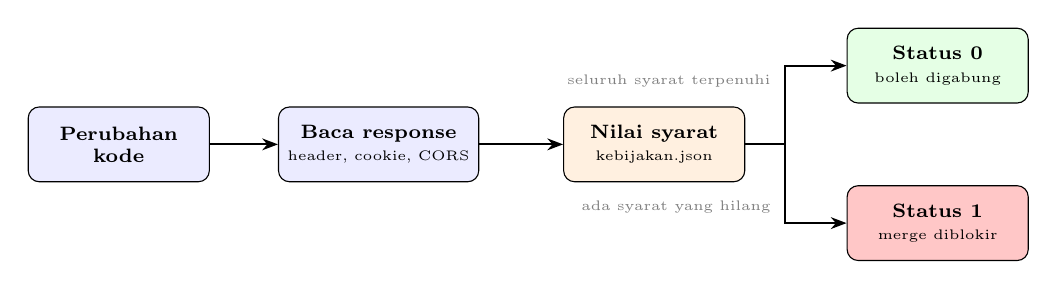
\begin{tikzpicture}[
    font=\scriptsize,
    kotak/.style={draw, rounded corners, minimum height=0.95cm,
                  minimum width=2.3cm, align=center, font=\scriptsize\bfseries},
    panah/.style={-{Stealth[length=2mm]}, thick}
  ]
    \node[kotak, fill=blue!8] (ubah) at (0,0) {Perubahan\\kode};
    \node[kotak, fill=blue!8] (baca) at (3.3,0) {Baca response\\{\tiny\mdseries header, cookie, CORS}};
    \node[kotak, fill=orange!12] (nilai) at (6.8,0) {Nilai syarat\\{\tiny\mdseries kebijakan.json}};
    \node[kotak, fill=green!10] (gabung) at (10.4,1.0) {Status 0\\{\tiny\mdseries boleh digabung}};
    \node[kotak, fill=red!22] (tolak) at (10.4,-1.0) {Status 1\\{\tiny\mdseries merge diblokir}};

    \draw[panah] (ubah) -- (baca);
    \draw[panah] (baca) -- (nilai);
    \draw[panah] (nilai.east) -- ++(0.5,0) |- (gabung.west);
    \draw[panah] (nilai.east) -- ++(0.5,0) |- (tolak.west);
    \node[font=\tiny, gray, anchor=east] at (8.4,0.8) {seluruh syarat terpenuhi};
    \node[font=\tiny, gray, anchor=east] at (8.4,-0.8) {ada syarat yang hilang};
  \end{tikzpicture}

  \vspace{12pt}
  {\small Yang dinilai adalah \textit{response} yang benar-benar dikirim
  aplikasi, bukan pembacaan kodenya.}
\end{frame}

\begin{frame}[fragile]{{\Large Membaca Verdict Gate}}
  \vspace{2pt}
\begin{lstlisting}[language=bash]
python periksa-keamanan.py

# Keluarannya:
#   Pemeriksaan                                  Keadaan      Verdict
#   / Content-Security-Policy                    sesuai       lolos
#   / X-Content-Type-Options                     sesuai       lolos
#   / Referrer-Policy                            sesuai       lolos
#   / Permissions-Policy                         sesuai       lolos
#   cookie sesi HttpOnly                         sesuai       lolos
#   cookie sesi SameSite=Lax                     sesuai       lolos
#   CORS izin untuk https://toko.pradita.ac.id   sesuai       lolos
#   CORS tolak https://situs-lain.example        sesuai       lolos
#
# Lolos: seluruh syarat keamanan terpenuhi.
\end{lstlisting}
\end{frame}

\begin{frame}{{\Large Gate yang Selalu Lolos Tidak Membuktikan Apa Pun}}
  \vspace{6pt}
  \centering
  {\footnotesize
  \begin{tabularx}{\textwidth}{Yrrr}
    \hline
    \textbf{Sasaran} & \textbf{Syarat} & \textbf{Lolos} & \textbf{Status keluar} \\
    \hline
    Aplikasi Bab 7 & 18 & 18 & 0 \\
    \hline
    Server statis bawaan Python & 9 & 1 & 1 \\
    \hline
  \end{tabularx}}

  \vspace{8pt}
  {\small Satu baris justru lolos pada pembanding: syarat "origin tak
  terdaftar tidak menerima izin" terpenuhi karena server itu memang tidak
  pernah mengirim header CORS. Syarat berbentuk larangan perlu dipasangkan
  dengan syarat positifnya.}
\end{frame}

\section{Persiapan Latihan}

\begin{frame}{\hfill}
  \centering
  \Huge{\textbf{Persiapan Latihan}}
\end{frame}

\begin{frame}[fragile]{{\Large Basis Data, Venv, dan Aturan Main}}
  \vspace{2pt}
\begin{lstlisting}[language=bash]
cd sources/chapter07
docker compose up -d
./siapkan-data.sh
python3 -m venv ../.venv
../.venv/bin/pip install "psycopg[binary]" ruff pip-audit
\end{lstlisting}
  \vspace{4pt}
  {\small Seluruh pemeriksaan bersifat mengamati dan hanya diarahkan ke
  aplikasi yang berjalan di komputer sendiri. Tidak ada perintah di bab ini
  yang boleh diarahkan ke situs kampus maupun sistem milik orang lain.}
\end{frame}

\section{Latihan 1: Header Keamanan}

\begin{frame}{\hfill}
  \centering
  \Huge{\textbf{Latihan 1\\Membaca Header Keamanan}}
\end{frame}

\begin{frame}{{\Large Langkah Kerja}}
  \vspace{8pt}
  \begin{enumerate}
    \item Nyalakan aplikasinya, lalu nyalakan juga server statis bawaan
          Python di port 8031 sebagai pembanding.
    \item Baca header kedua server dengan \texttt{curl}, lalu catat
          perbedaannya.
    \item Tambahkan satu header baru ke \texttt{kebijakan.json}, misalnya
          \texttt{X-Frame-Options} bernilai \texttt{DENY}, nyalakan ulang
          aplikasinya, lalu periksa kembali.
  \end{enumerate}
\end{frame}

\begin{frame}[fragile]{{\Large Membaca Header Dua Server}}
  \vspace{2pt}
\begin{lstlisting}[language=bash]
SECRET_SESI=rahasia-latihan python aplikasi.py &
(cd statis && python -m http.server 8031 &)
curl -sI http://127.0.0.1:8030/ | grep -iE "^(content-security|x-content)"
curl -sI http://127.0.0.1:8031/index.html | grep -iE "^(content-security)"

# Keluarannya:
# Content-Security-Policy: default-src 'self'
# X-Content-Type-Options: nosniff
\end{lstlisting}
  \vspace{2pt}
  {\footnotesize Perintah terakhir tidak mengeluarkan apa pun, karena server
  bawaan memang tidak mengirim header itu.}
\end{frame}

\begin{frame}{{\Large Contoh Hasil dan Lembar Isian Latihan 1}}
  \vspace{4pt}
  \centering
  {\footnotesize
  \begin{tabularx}{\textwidth}{Yll}
    \hline
    \textbf{Header} & \textbf{Server bawaan} & \textbf{Aplikasi Bab 7} \\
    \hline
    \texttt{Content-Security-Policy} & tidak ada & \texttt{default-src 'self'} \\
    \hline
    \texttt{X-Content-Type-Options} & tidak ada & \texttt{nosniff} \\
    \hline
  \end{tabularx}}

  \vspace{6pt}
  \centering
  {\footnotesize
  \begin{tabularx}{\textwidth}{Yll}
    \hline
    \textbf{Header} & \textbf{Server bawaan} & \textbf{Aplikasi Bab 7} \\
    \hline
    Keempat header wajib & \dots & \dots \\
    \hline
    Header tambahan pilihan sendiri & \dots & \dots \\
    \hline
  \end{tabularx}}

  \vspace{4pt}
  {\footnotesize Pertanyaan: header mana yang membatasi asal skrip, mengapa
  header dipasang di satu fungsi, dan apa yang terjadi pada header baru tanpa
  aplikasinya dinyalakan ulang?}
\end{frame}

\section{Latihan 2: Cookie dan CORS}

\begin{frame}{\hfill}
  \centering
  \Huge{\textbf{Latihan 2\\Cookie dan Lintas Origin}}
\end{frame}

\begin{frame}{{\Large Langkah Kerja}}
  \vspace{8pt}
  \begin{enumerate}
    \item Baca header \texttt{Set-Cookie} dari alamat profil, catat tiap
          atributnya.
    \item Minta alamat yang sama tiga kali dengan header \texttt{Origin}
          berbeda, catat header izin yang kembali.
    \item Tambahkan satu origin baru ke daftar di \texttt{kebijakan.json},
          nyalakan ulang aplikasinya, lalu ulangi pemeriksaannya.
  \end{enumerate}
\end{frame}

\begin{frame}[fragile]{{\Large Membaca Cookie dan Izin Origin}}
  \vspace{2pt}
\begin{lstlisting}[language=bash]
curl -sI http://127.0.0.1:8030/api/profil | grep -i "^set-cookie"
curl -sI -H "Origin: https://toko.pradita.ac.id" \
  http://127.0.0.1:8030/api/profil | grep -i "^access-control"
curl -sI -H "Origin: https://situs-lain.example" \
  http://127.0.0.1:8030/api/profil | grep -iE "^(access-control|vary)"

# Keluarannya:
# Set-Cookie: sesi=...; HttpOnly; SameSite=Lax; Path=/; Max-Age=3600
# Access-Control-Allow-Origin: https://toko.pradita.ac.id
# Vary: Origin
\end{lstlisting}
\end{frame}

\begin{frame}{{\Large Lembar Isian Latihan 2}}
  \vspace{6pt}
  \centering
  {\footnotesize
  \begin{tabularx}{\textwidth}{lY}
    \hline
    \textbf{Yang diperiksa} & \textbf{Hasilnya} \\
    \hline
    Atribut cookie sesi & \dots \\
    \hline
    Origin terdaftar pertama & \dots \\
    \hline
    Origin terdaftar kedua & \dots \\
    \hline
    Origin tidak terdaftar & \dots \\
    \hline
    Origin baru yang ditambahkan sendiri & \dots \\
    \hline
  \end{tabularx}}

  \vspace{6pt}
  {\footnotesize Pertanyaan: siapa yang sebenarnya dilindungi aturan CORS,
  mengapa nilai bintang tidak dipakai, dan mengapa \texttt{Vary: Origin}
  tetap dikirim walaupun izinnya tidak diberikan?}
\end{frame}

\section{Latihan 3: Teks sebagai Data}

\begin{frame}{\hfill}
  \centering
  \Huge{\textbf{Latihan 3\\Teks Pengguna sebagai Data}}
\end{frame}

\begin{frame}[fragile]{{\Large Langkah Kerja dan Perintahnya}}
  \vspace{2pt}
\begin{lstlisting}[language=bash]
curl -s "http://127.0.0.1:8030/api/cari?judul=Pengantar%20Jilid%207" | head -c 80
curl -s --get --data-urlencode "judul=Pengantar'; SELECT 1 --" \
  http://127.0.0.1:8030/api/cari | head -c 80
curl -s --get --data-urlencode 'nama=<b>Mahasiswa</b>' \
  http://127.0.0.1:8030/sapa | grep -i halo

# Keluarannya:
# {"kata_kunci": "Pengantar Jilid 7", "hasil": [{"id": ...
# {"kata_kunci": "Pengantar'; SELECT 1 --", "hasil": []}
# <body><h1>Halo, &lt;b&gt;Mahasiswa&lt;/b&gt;</h1>
\end{lstlisting}
\end{frame}

\begin{frame}{{\Large Contoh Hasil dan Lembar Isian Latihan 3}}
  \vspace{4pt}
  \centering
  {\footnotesize
  \begin{tabularx}{\textwidth}{Yrl}
    \hline
    \textbf{Yang dikirim} & \textbf{Baris} & \textbf{Status} \\
    \hline
    \texttt{Pengantar Jilid 7} & 20 & 200 \\
    \hline
    \texttt{Pengantar'; SELECT 1 -{}-} & 0 & 200 \\
    \hline
  \end{tabularx}}

  \vspace{6pt}
  \centering
  {\footnotesize
  \begin{tabularx}{\textwidth}{Yrl}
    \hline
    \textbf{Yang dikirim} & \textbf{Baris} & \textbf{Status} \\
    \hline
    Kata kunci biasa & \dots & \dots \\
    \hline
    Kata kunci bertanda baca & \dots & \dots \\
    \hline
    Nama berisi tanda kurung siku & \dots & \dots \\
    \hline
  \end{tabularx}}

  \vspace{4pt}
  {\footnotesize Pertanyaan: mengapa pencarian kedua menghasilkan nol baris,
  dan apa bedanya menolak teks tertentu dengan memperlakukan seluruh teks
  sebagai data?}
\end{frame}

\section{Latihan 4: Gate Keamanan}

\begin{frame}{\hfill}
  \centering
  \Huge{\textbf{Latihan 4\\Menegakkan Gate Keamanan}}
\end{frame}

\begin{frame}{{\Large Langkah Kerja}}
  \vspace{6pt}
  \begin{enumerate}
    \item Baca \texttt{kebijakan.json}, tulis dugaan berapa syarat yang akan
          terpenuhi aplikasi dan berapa pada server pembanding.
    \item Jalankan gerbangnya terhadap keduanya, catat jumlah syarat, jumlah
          yang lolos, dan status keluarnya.
    \item Jalankan pemeriksaan dependensi dan analisis statis, catat jumlah
          temuannya.
    \item Hapus sementara satu header dari \texttt{kebijakan.json}, nyalakan
          ulang aplikasinya, jalankan ulang gerbangnya, lalu kembalikan.
  \end{enumerate}
\end{frame}

\begin{frame}[fragile]{{\Large Menjalankan Gate pada Dua Sasaran}}
  \vspace{2pt}
\begin{lstlisting}[language=bash]
python periksa-keamanan.py
echo $?
python periksa-keamanan.py kebijakan-pembanding.json
echo $?
./audit-dependensi.sh
ruff check .

# Keluarannya:
# Lolos: seluruh syarat keamanan terpenuhi.
# 0
# Gagal: 8 syarat keamanan belum terpenuhi.
# 1
# No known vulnerabilities found
# All checks passed!
\end{lstlisting}
\end{frame}

\begin{frame}{{\Large Contoh Hasil dan Lembar Isian Latihan 4}}
  \vspace{4pt}
  \centering
  {\footnotesize
  \begin{tabularx}{\textwidth}{Yrrr}
    \hline
    \textbf{Sasaran} & \textbf{Syarat} & \textbf{Lolos} & \textbf{Status keluar} \\
    \hline
    Aplikasi Bab 7 & 18 & 18 & 0 \\
    \hline
    Server statis bawaan Python & 9 & 1 & 1 \\
    \hline
  \end{tabularx}}

  \vspace{6pt}
  \centering
  {\footnotesize
  \begin{tabularx}{\textwidth}{Yrrr}
    \hline
    \textbf{Sasaran} & \textbf{Syarat} & \textbf{Lolos} & \textbf{Status keluar} \\
    \hline
    Aplikasi Bab 7 & \dots & \dots & \dots \\
    \hline
    Server statis bawaan Python & \dots & \dots & \dots \\
    \hline
    Aplikasi dengan satu header dihapus & \dots & \dots & \dots \\
    \hline
  \end{tabularx}}

  \vspace{4pt}
  {\footnotesize Pertanyaan: mengapa gerbang menilai \textit{response} dan
  bukan kodenya, mengapa satu syarat justru lolos pada pembanding, dan
  mengapa hasil pemeriksaan dependensi punya umur simpan?}
\end{frame}

\begin{frame}[fragile]{{\Large Membersihkan}}
  \vspace{2pt}
\begin{lstlisting}[language=bash]
docker compose down -v
\end{lstlisting}
  \vspace{6pt}
  {\small Opsi \texttt{-v} ikut menghapus volume datanya, sehingga penyiapan
  berikutnya dimulai dari keadaan bersih.}
\end{frame}

\section{Ringkasan}

\begin{frame}{\hfill}
  \centering
  \Huge{\textbf{Ringkasan}}
\end{frame}

\begin{frame}{{\Large Ringkasan}}
  \vspace{8pt}
  \begin{itemize}
    \item Model ancaman menghasilkan satu batas kepercayaan dan tiga
          kewajiban, bukan daftar serangan.
    \item Empat header keamanan dikirim lewat satu fungsi. Server bawaan
          Python tidak mengirim satu pun dari keempatnya.
    \item Cookie sesi memakai \texttt{HttpOnly} dan \texttt{SameSite=Lax},
          dan izin lintas origin hanya diberikan kepada daftar di file
          kebijakan.
    \item Teks pengguna tetap data: kata kunci bertanda kutip dijawab 200
          dengan nol baris, dan markup tampil sebagai huruf.
    \item Gerbang menilai 18 syarat dan keluar dengan status 0, sedangkan
          server tanpa penyetelan meloloskan 1 dari 9 dan keluar status 1.
  \end{itemize}
\end{frame}

\end{document}
